\chapter{Gráficas Helly}
Uno de los resultados más importantes entorno a gráficas buenas fue probado por Erich Prisner en 1988 en su artículo ``Convergence of iterated clique graphs'' publicado en 1992 por la revista Discrete Mathematics, dicho resultado fue deducido como corolario de un teorema probado por el topólogo Clifford Hugh Dowker en 1952 en su artículo ``Homology Groups of Relations'' publicado por la revista The Annals of Mathematics.
El teorema de Prisner nos permite determinar un conjunto de gráficas en el que la homotopía es invariante bajo el operador de clanes.

El propósito de este capítulo es reconstruir la demostración desde el inicio, enumerando todos los teoremas necesarios junto con su demostración. Para ver las demostraciones originales el lector puede consultar ....

\section{Gráficas Helly}
Las gráficas que nos interesan en este capítulo son las gráficas que cumplen la propiedad de ser clan-Helly, en está sección las estudiaremos más a detalle, a continuación se enuncia su definición.
\begin{Defi}[Gráficas clan-Helly]
Una gráfica G es clan-Helly si su colección de clanes $\mathcal{C}(G)$ cumple que cualquier subcolección de $\mathcal{C}(G)$ con la propiedad de que cualesquiera dos clanes tienen intersección no vacía, tiene intersección no vacia.  
\end{Defi}

Para estudiar estas gráficas, una herramienta útil es centrarnos en su contraparte, preguntandonos que debe pasar para que una gráfica no sea clan-Helly. Así de la definición se sigue que la gráfica que buscamos debe tener al menos tres clanes $\{q_1,q_2,q_3\}$ que se intersequen dos a dos y tengan interseccción vacía.


\begin{center}
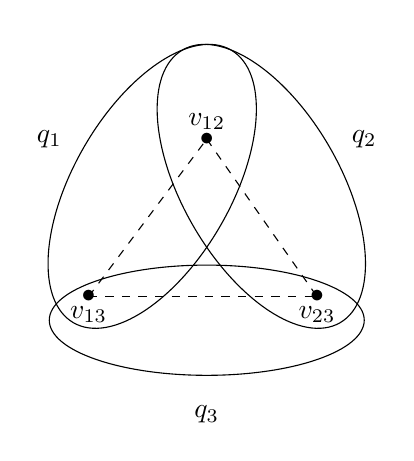
\begin{tikzpicture}
%\draw (-4,-4) grid (4,4);
\draw [rotate=60] (0,0.8) ellipse (2 and 1);
\draw [rotate=300] (0,0.8) ellipse (2 and 1);
\draw  (0,-1.3) ellipse (2 and 0.7);
\draw (-2,1) node {$q_1$}; 
\draw (2,1) node {$q_2$}; 
\draw (0,-2.5) node {$q_3$};
\draw (0,1) node {$\bullet$}; 
\draw (1.4,-1) node {$\bullet$}; 
\draw (-1.5,-1) node {$\bullet$}; 
\draw (0,1) node [above]{$v_{12}$}; 
\draw (1.4,-1) node[below] {$v_{23}$}; 
\draw (-1.5,-1) node [below] {$v_{13}$};
\draw  [dashed](0,1) -- (1.4,-1);
\draw  [dashed](-1.5,-1) -- (1.4,-1);
\draw  [dashed](-1.5,-1) -- (0,1);
\end{tikzpicture}
\end{center}
Notemos que los vértices $v_{12}$, $v_{13}$ y $v_{23}$ forman una completa, por lo que los clanes $q_1$, $q_2$ y $q_3$ deben tener al menos tres vértices cada uno. La manera más sencilla, tenendo el menor número de aristas y vértices sería que los clanes $q_1$, $q_2$ y $q_3$ tuvieran exactamente tres vértices cada uno, así la completa $\{v_{12}, v_{13}, v_{23}\}$ sería también un clan, teniendo en total cuatro clanes, seis vértices y nueve aristas.
\begin{figure}[H]\label{pequenh}
\centering
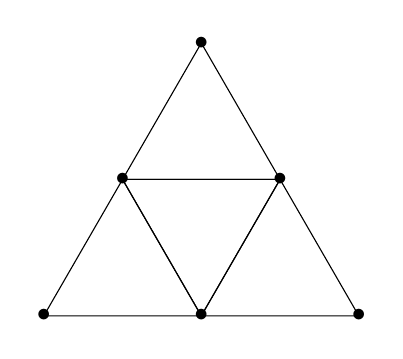
\begin{tikzpicture}
\draw (-2,0) -- (0,0) -- (-1,1.73205) -- cycle;
\draw (0,0) -- (-1,1.73205) --(1,1.73205) -- cycle;
\draw (0,0) -- (2,0) --(1,1.73205)  -- cycle;
\draw (-1,1.73205) -- (1,1.73205) --(0,3.4641)  -- cycle;
\draw (-2,0) node {$\bullet$};
%\draw (0,0) node[below] {1};
\draw (0,0) node {$\bullet$};
%\draw (1,0) node[below] {2};
\draw (2,0) node {$\bullet$};
%\draw (2,0) node[below] {3};
\draw (-1,1.73205) node {$\bullet$};
%\draw (0.5,0.86602) node[left] {4};
\draw (1,1.73205) node {$\bullet$};
%\draw (1.5,0.86602) node[right] {5};
\draw (0,3.4641) node {$\bullet$};
%\draw (1,1.73205) node[above] {6};
\end{tikzpicture}
\caption{Gráfica más pequeña que no es clan-Helly}
\end{figure}
Es posible extender los clanes de muchas maneras, siempre y cuando cada nuevo vértice que se agregue pertenezca a lo más a dos clanes del conjunto $\{q_1,q_2,q_3\}$.
Esta idea es de gran utilidad para dar una caracterización de las gráficas clan-Helly, para ello introduciremos la siguiente definición.
\begin{Defi}[Triángulo extendido]
Dada una completa $T$ de tres vértices de una gráfica $G$, decimos que $T$ es un triángulo y definimos el triángulo extendido $\hat{T}$ de $T$, como la subgráfica de $G$ inducida por los vértices que son adyacentes a al menos dos vértices de $T$.   
\end{Defi}

 
\begin{Teo}
Sea G una gráfica. Los siguientes enunciados son equivalentes:
\begin{enumerate}
\item G es clan Helly.
\item Para todo triángulo T de G, $\hat{T}$ es un cono.
\end{enumerate}
\end{Teo}
\begin{Dem}
...
\end{Dem}
\section{Subdivisión baricéntrica}
En esta sección estudiaremos la primera subdivisión baricéntrica de una gráfica G, que consiste de un complejo siplicial abstracto definido a partir de darle un orden parcial por contención a los simplejos de la gráfica. La primera subdivisión baricéntrica es muy importante ya que es homeomorfa a $\Delta(G)$ lo cual se demostrará en esta sección.

En general la primera subdivisión baricéntrica se puede definir para cualquier complejo simplicial abstracto y en el caso de complejos simpliciales en $\mathbb{R}^N$ se utiliza precisamente el baricentro de cada simplejo de ahí el nombre.

Antes de definir la subdivisión barecéntrica es necesario introducir las siguientes definiciones:

\begin{Defi}[Copo de simplejos]
Sea $\Delta$ una complejo simplicial abstracto, el copo de simplejos de $\Delta$ es el conjunto parcialmente ordenado definido como $P(\Delta) = (\Delta,\subseteq)$. 
\end{Defi}

\begin{Defi}[Complejo ordenado]
Sea $P$ un conjunto parcialmente ordenado, el complejo ordenado de $P$, denotado por $\Delta(P)$, es el complejo simplicial abstracto formado por las cadenas no vacías en $P$.
\end{Defi}
\begin{Defi}[Primera subdivisión baricéntrica]
Sea $\Delta$ un complejo simplicial abstracto, definimos la primera subdivisión baricéntrica de $\Delta$ como el complejo ordenado $sd\Delta = \Delta(P(\Delta))$.
\end{Defi}
\begin{Ejem}
Sea $\Delta = \{\{1\},\{2\},\{3\},\{1,2\},\{1,3\},\{2,3\},\{1,2,3\}\}$, el copo de simplejos de $\Delta$, $P(\Delta)$, se obtiene de asignar un orden por contención a $\Delta$, con lo que se forman las siguientes cadenas maximales:
\begin{align*}
&\{1\}\leq\{1,2\}\leq\{1,2,3\}\\
&\{1\}\leq\{1,3\}\leq\{1,2,3\}\\
&\{2\}\leq\{1,2\}\leq\{1,2,3\}\\
&\{2\}\leq\{2,3\}\leq\{1,2,3\}\\
&\{3\}\leq\{1,3\}\leq\{1,2,3\}\\
&\{3\}\leq\{2,3\}\leq\{1,2,3\}
\end{align*}
Luego el complejo ordenado de $P(\Delta)$, denotado por $\Delta(P(\Delta))$ es el conjunto que contiene todas las cadenas en $P(\Delta)$, teniendo un total de 25 elementos.
\end{Ejem}

\begin{Defi} 
El nervio de una familia de subconjuntos ${\{A_i\}}_{i\in I}$, denotado por $\mathcal{N}(A_i)$, es el complejo simplicial abstracto definido sobre los vértices $I$ tal que un subconjunto finito $\sigma \subseteq I$ está en $\mathcal{N}(A_i)$ si y sólo si ${\cup}_{i\in \sigma}A_i \neq \emptyset$
\end{Defi}
\begin{Ejem}
Sea G una gráfica, consideremos la colección de clanes de G, $\mathcal{C}(G) = \{q_1,...,q_n\}$, indizada por $I =\{1,...,n\}$, esta notación nos permite definir el nervio de la colleción de clanes $\mathcal{N}(q_i)$. Notemos que $\sigma = \{i_1,...,i_r\}$ pertenece a $\mathcal{N}(q_i)$ si y solo si $\cup_{k=1}^{r}q_{i_k}\neq\emptyset$, lo que implica que $\{q_{i_1},...,q_{i_r}\}$ es una completa de K(G), de donde se sigue que $\{q_{i_1},...,q_{i_r}\}$ pertenece a $\Delta(K(G))$.

Por lo tanto $\mathcal{N}(q_i)$ es isomorfo a un subcomplex de $\Delta(K(G))$, por simplicidad denotaremos a $\mathcal{N}(q_i)$ como $\mathcal{N}(G)$ y diremos que $\mathcal{N}(G)\subseteq \Delta(K(G))$.
\end{Ejem}

\begin{Teo}
Sea $\Delta$ un complejo simplicial abstracto, $\Delta$ y $sd\Delta$ son homeomorfos.
\end{Teo}

\begin{Dem}
Los vértices de un simplejo en $sd\Delta$ son simplejos de $\Delta$ de la forma $\{\sigma_0,\sigma_1,...,\sigma_n\}$ tales que $\sigma_0\subset \sigma_1\subset..\subset\sigma_n$.

Si consideramos la función 
\begin{equation*}
\sigma_{i} \rightarrow b_{\sigma_{i}}
\end{equation*}
Donde $b_{\sigma_{i}}$ es el baricentro de $\sigma_{i}$.
Como $\sigma_{i}$ es un conjunto convexo, se tiene que $b_{\sigma_{i}}$ pertenece a $\sigma_{i}$, además se tiene que $b_{\sigma_{i}}$ pertecene a $\sigma_{n}$.
\end{Dem}
